\chapter { مرور }

%{
%در این فصل برای پیا‌ده‌سازی سیستم انیمیشن به دنبال ارضا کردن 4 هدف کلی هستیم.
%\begin{enumerate}
%	\item نمایش اسکلت شخصیت در یک محیط سه‌بعدی
%	\item نمایش انیمیشن‌های سه‌بعدی اسکلت
%	\item نمایش شخصیت دارای مدل و اجرای انیمیشن بر روی آن
% 	\item با پیاده‌سازی روش ترکیب برای ترکیب انیمیشن‌های مختلف با یکدیگر
%\end{enumerate}


از گذشته تا امروز نحوه‌ی تولید و همچنین استفاده از کلیپ‌های پویانمایی تغییرات زیادی کرده است.
در گذشته اکثر پویانمایی‌ها با استفاده از دست و ترسیم بر روی صفحات سلولوئیدی تولید می‌شدند.
درصورتیکه که امروزه، اکثر کلیپ‌های پویانمایی توسط تصاویر گرافیکی کامپیوتری ساخته‌می‌شوند.
اگرچه با پیشرفت تکنولوژی روش‌های جدیدی برای تولید پویانمایی به‌وجودآمده، همچنان نیز از اکثر روش‌هایی که در 
پویانمایی سنتی استفاده می‌شد در پویانمایی کامپیوتری نیز استفاده می‌شود.

امروزه نه تنها از پویانمایی برای تولید فیلم و کارتون، استفاده می‌شود، بلکه آن‌ها نقش 
تاثیرگذاری در بازی‌های کامپیوتری پیدا کرده‌اند.
برای تولید بازی‌های کامپیوتری از موتور‌های بازی‌سازی استفاده می‌شود.
موتور‌های بازی‌سازی دارای مولفه‌های متفاوتی هستند که هرکدام وظیفه‌ی مخصوص به خودشان را دارند.
مولفه‌ای که وظیفه‌ی پخش کلیپ‌های پویانمایی را دارد، مولفه‌ی پویانمایی گویند.
بدیهی است اگر بخواهیم از سیستم پویانمایی استفاده کنیم نیازمند یک محیط گرافیکی هستیم.
محیط‌های گرافیکی به صورت معمول از کارت گرافیک استفاده می‌کنند. برای دسترسی به توابع 
کارت گرافیکی می‌توان از یک رابط کاربری مانند 
\lr{DirectX}
یا
\lr{OpenGL}
استفاده کرد.
علاوه بر این برای مشاهده‌ی اشیاء موجود در محیط سه‌بعدی نیاز است که محیط را نورپردازی کنیم.
روش‌های متنوعی برای نورپردازی محیط وجود دارند. یکی از این روش‌ها 
\lr{Phong Shading}
است که در این پروژه نیز استفاده شده است.

در اکثر سیستم‌های پویانمایی بازی‌های کامپیوتری از پویانمایی اسکلتی برای پخش و ترکیب کلیپ‌های پویانمایی 
استفاده می‌شود.

پویانمایی اسکلتی تکنیکی در پویانمایی کامپیوتری است که به وسیله‌ی آن، شخصیت‌های درون بازی متحرک می‌شوند. 
این سیستم به دو بخش کلی تقسیم می‌شود.
یک بخش،یک مش یا پوسته است که برای به نمایش کشاندن شخصیت در محیط سه‌بعدی استفاده می‌شود و بخش دوم یک اسکلت است. این اسکلت مجموعه سلسله مراتبی از قطعات به‌‌هم‌پیوسته است که به هر قطعه یک مفصل گویند.
در این تکنیک، اسکلت شخصیت درون بازی متحرک شده و با روش‌های موجود، پوسته یا مش آن شخصیت، اسکلت را دنبال می‌کند.


در این فصل، ابتدا مروری بر پویانمایی سنتی و روش‌های تولید آن می‌کنیم. سپس نگاهی به 
پیشرفت صنعت تولید پویانمایی کامپیوتری می‌اندازیم و روش‌های فعلی تولید پویانمایی را خواهیم گفت.
پس از آن توضیحی در رابطه با موتور‌های بازی‌سازی و به ویژه موتور آنریل خواهیم داد.

در قسمت انتهایی توضیحی در مورد 
\lr{Phong Shading}
که یکی از روش‌های نورپردازی محیط سه‌بعدی است خواهیم داد و علاوه بر آن
در انتها توضیحات جامعی را در مورد پویانمایی اسکلتی ارائه خواهیم کرد

\section{تاریخچه‌ی پویانمایی سنتی}

پویانمایی سنتی که با اسم‌های مختلفی مانند "پویانمایی مرسوم" ، "پویانمایی سل‌ای"و "پویانمایی بادست" شناخته می‌شود، روشی 
غالب برای تولید فیلم‌های پویانمایی‌شده در حدود قرن 20 میلادی بود.
در این روش، به صورت کلی پویانمایی به وسیله‌ی نقاشی با دست به وجود می‌آید.
درواقع هر فریم از فیلم، یک عکس از نقاشی است و
برای به وجود آوردن توهم حرکت، هر نقاشی اندکی با نقاشی قبلی خود تفاوت دارد.

برای تولید پویانمایی سنتی، از روش‌های مختلفی استفاده می‌شد. در اینجا به بررسی
سه روش استفاده شده در پویانمایی سنتی می‌پردازیم.

\subsection{فریم‌های کلیدی و درمیان}
از آنجایی که تولید پویایی با دست و کشیدن نقاشی کار بسیار طولانی‌ای بود، برای اینکه وقت پویانمای‌های ارشد 
ذخیره شود، این پویانماها فریم‌های اصلی یک حرکت را بر روی کاغذ ترسیم می‌کردند و 
فریم‌های میانی را پویانماهای جوان پر می‌کردند.
 
\begin{figure}[ht]
	\centerline{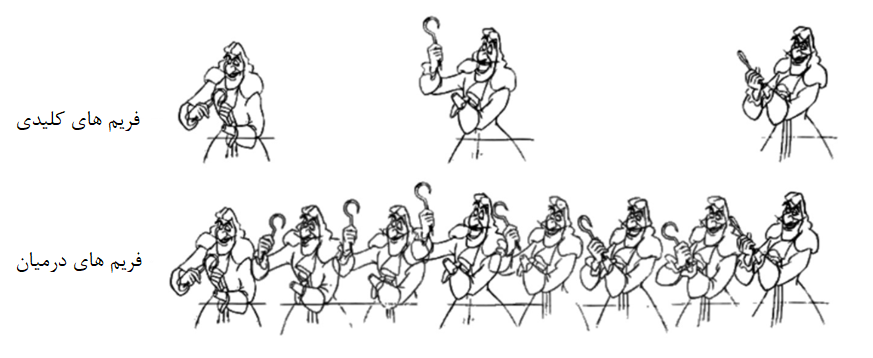
\includegraphics[width=\textwidth,height=\textheight,keepaspectratio]{Figures/Ch1/KeyframeAnimation.png}}

	\caption{فریم‌های کلیدی و درمیان}
	\label{fig:KeyframeAnimation}
\end{figure}

\subsection{چشم‌انداز چندمنظوره}

استفاده از چشم‌انداز چندمنظوره روش دیگری بود که در پویانمایی سنتی استفاده می‌شد.
هماطور که از تصویر زیر مشخص است، برای نمایش یک محیط از یک چشم‌انداز استفاده می‌شد.
این چشم‌انداز می‌توانست نشان دهنده‌ی قرارگیری محیط در فواصل مختلف باشد. در این صورت، زمانی که 
دوربین در صحنه حرکت می‌کرد این توهم را در مخاطب ایجاد می‌کرد که گویی در محیط در حال حرکت هستیم.

\begin{figure}[ht]
	\centerline{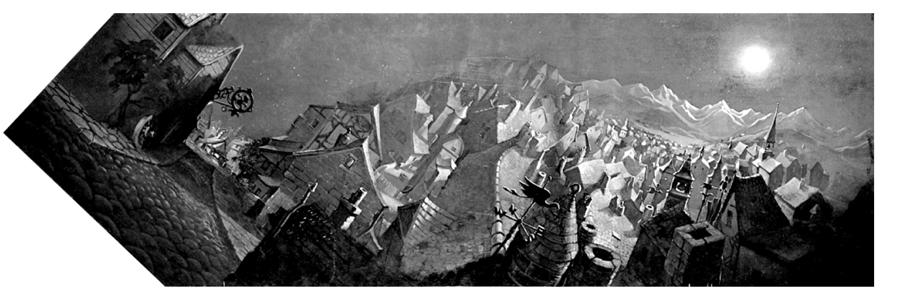
\includegraphics[width=\textwidth,height=\textheight,keepaspectratio]{Figures/Ch1/Panorama.png}}

	\caption{چشم‌انداز چندمنظوره}
	\label{fig:Panorama}
\end{figure}


\subsection{لایه‌های مختلف}

با استفاده از این روش، پویانما‌ها یک صحنه را به چند قسمت مختلف تقسیم می‌کردند.
به عنوان مثال لایه‌های مختلفی برای هر شخصیت درون صحنه استفاده می‌شد. علاوه برا ین یک لایه نیز برای تصویر پس‌زمینه استفاده می‌شد.
از آنجایی که این لایه‌ها یک صفحه‌ی شفاف هستند بنابراین می‌توان لایه‌‌ها را 
بر روی هم انباشته کرد و با تصویر برداری از بالا تمام صحنه را تصویربرداری کرد.
این روش در تصویر 
\ref{fig:DifferentLayers}
آورده شده است.

\begin{figure}[ht]
	\centerline{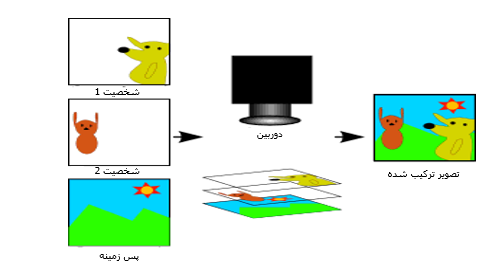
\includegraphics[width=\textwidth,height=\textheight,keepaspectratio]{Figures/Ch1/DifferentLayers.png}}

	\caption{لایه‌های مختلف}
	\label{fig:DifferentLayers}
\end{figure}

\section{پویانمایی کامپیوتری}

اگر بخواهیم نگاهی به تاریخچه‌ی انیمیشن‌های کامپیوتری بیاندازیم، مشاهده می‌کنیم که 
در حدود دهه‌ی 1980 میلادی شرکت دیزنی به عنوان یکی از اولین شرکت‌های جهان، شروع به 
دیجیتالی کردن خط لوله‌ی تولید پویانمایی سنتی خود کرد.
در این دیجیتال‌سازی بسیاری از روش‌ها و ایده‌‌های استفاده شده در پویانمایی سنتی،
به‌کار گرفته‌شد.
اولین مقالات این حوزه توسط آقای جان لستر از کارمندان پیکسار به عنوان 
"اصول پویانمایی سنتی به‌کار رفته در پویانمایی کامپیوتری سه‌بعدی"
ارائه شد.
در این مقاله اصول اولیه پویانمایی سنتی دوبعدی ترسیم شده با دست
و کاربرد آن‌ها در پویانمایی کامپیوتری سه‌بعدی شرح داده شده است.
\cite{Lasseter1987animation}
 
پویانمایی کامپیوتری تنها محدود به دنیای سینما و فیلم‌های پویانمایی نمی‌شوند و به دنیای
بازی‌های کامپیوتری نیز ورود پیدا کرده‌اند. بازی‌های کامپیوتری سعی می‌کنند دیوار میان تماشاگران و فیلم را بشکنند و 
با تعاملی بودن و دادن آزادی عمل به بازیکن، سعی می‌کنند داستان را به گونه‌ای تعریف کنند که گویی بازیکن یکی از شخصیت‌های اصلی داستان است.
پویانمایی در بازی‌های کامپیوتری اهمیت بسیار بالایی دارد زیرا همانطور که گفته شد باعث 
جان بخشیدن به شخصیت‌ها می‌شود که اهمیت بسیار بالایی برای جلب توجه بازیکنان در هنگام داستان‌سرایی دارد.

با پیشرفت تکنولوژی، همراه با استفاده از روش‌های گذشته، روش‌های جدیدتری برای تولید پویانمایی توسعه یافته‌است که 
در ادامه به چند مورد از آن‌‌ها می‌پردازیم.

\subsection{فریم‌های کلیدی و درمیان}

همانطور که اشاره شد در پویانمایی کامپیوتری از روش‌های موجود در 
پویانمایی سنتی استفاده شده است. در اینجا نیز فریم‌های کلیدی 
یک حرکت توسط پویانماها به وجود می‌‌آیند ولی فریم‌های میانی به جای اینکه توسط پویانماها به وجود آیند،
توسط کامپیوتر با استفاده از روش های درون‌یابی به وجود می‌آیند.

\subsection{رویه}

در این روش، حرکت بر اساس یک الگوریتم بیان می‌شود.
درواقع انیمیشن‌ها در این نوع پویانمایی، توابعی با تعداد کمی از متغیر‌ها هستند.
به عنوان مثال یک تابعی را درنظر بگیرید که به گرفتن ورودی ثانیه، دقیقه و ساعت، 
یک شئ ساعت را خروجی دهد که عقربه‌هایش در جای مناسب با توجه به ورودی‌ها قرار گرفته باشد.
حال می‌توان با تغییر ورودی‌ها حرکت ساعت را شبیه‌سازی کنیم.

\subsection{مبتنی بر فیزیک}

پویانمایی مبتنی بر فیزیک پلی میان دنیای پویانمایی با 
دنیای واقعی است. در این روش با نسبت دادن ویژگی‌های فیزیک به اشیاء سه‌بعدی و سپس حل‌کردن
فرمول‌های فیزیک مانند فرمول حرکت یا فرمول‌های نیوتن،
فیزیک را شبیه سازی می‌کند.
پویانمایی‌های مبتنی بر فیزیک شخصیت را قادر می‌سازد تا حرکت‌های خود را 
به صورت پویا با محیط تنظیم کند.

\subsection{ضبط حرکت
\protect \LTRfootnote{Motion Capture}}

به فرآیند ثبت و دیجیتالی‌کردن حرکت یک شئ یا شخص، ضبط حرکت گویند.
ضبط حرکت توسط دوربین‌های مادون قرمز که تعدادی زیادی از آن‌ها در صحنه‌ی ضبط قرار دارند، صورت می‌گیرد.
این دوربین‌ها به صورت شبکه به یکدیگر متصل هستند و پس از کالیبره شدن، آماده‌ی استفاده هستند.
این دوربین‌ها با استفاده از نشانگر‌های سفیدی که بر روی لباس بازیگران 
ضبط حرکت قرار دارد، داده‌های مورد نیازشان را دریافت می‌کنند.
قابل ذکر است این نشانگر‌ها بازتابنده‌ی مادون قرمز هستند که توسط دوربین‌ها دریافت می‌شود.
در نهایت پویانماها به پاکسازی و پردازش این داده‌ها پرداخته تا آن را 
برای استفاده‌ی شخصیت‌های سه بعدی آماده کنند.




\section{موتور بازی‌سازی}
موتور‌های بازی‌سازی پلتفرم‌هایی هستند که ساخت بازی‌های رایانه‌ای را آسان‌تر می‌کنند.
آن ها به شما این امکان را می‌دهند تا عناصر بازی مانند پویانمایی، تعامل با کاربر یا تشخیص برخورد میان اشیاء را در یک واحد ادغام و ترکیب کنید.
\cite{barczak2019comparative}
زمانی که از اصطلاح موتور بازی‌سازی استفاده می‌کنیم منظورمان نرم‌افزارهای قابل توسعه‌ای هستند که می توانند پایه و اساس بسیاری از بازی‌های مختلف باشند.
\cite{GameEngineArchitecture}
موتورهای بازی‌سازی متشکل از اجزای مختلفی هستند که قابلیت‌های لازم برای ساخت بازی را فراهم می‌کنند.
رایج ترین اجزای موتور بازی عبارتند از:
\cite{barczak2019comparative}
\begin{itemize}
    \item[-] مولفه‌ی صدا: نقش اصلی این مولفه تولید جلوه‌های صوتی در بازی است.
    \item[-] موتور رندر: وظیفه اصلی این مولفه تبدیل داده‌های ورودی به پیکسل‌ها، برای به تصویر کشاندن بر روی صفحه است.
    \item[-] مولفه هوش مصنوعی: این مولفه مسئولیت ارائه‌ی تکنیک‌هایی برای تعریف قوانین رفتار شخصیت‌هایی را دارد که توسط بازیکنان کنترل نمی‌شوند.
    \item[-] مولفه پویانمایی: نقش اصلی این مولفه اجرای کلیپ‌های پویانمایی مختلف مانند حرکت است.
    \item[-] مولفه شبکه: وظیفه اصلی این مولفه قادرساختنِ بازیِ همزمانِ بازیکنان با یکدیگر، از طریق استفاده از دستگاه‌های متصل به اینترنت است.
    \item[-] مولفه منطق یا مکانیک بازی: این مولفه قوانین حاکم بر دنیای مجازی، ویژگی‌های شخصیت‌های بازیکنان، هوش مصنوعی و اشیاء موجود در دنیای مجازی و همچنین وظایف و اهداف بازیکنان را تعریف می‌کند.
    \item[-] ابزارهای نرم‌افزاری: وظیفه اصلی این ابزارها افزایش راندمان و سرعت تولید بازی با موتور بازی‌سازی است. آن‌ها توانایی اضافه‌کردن بسیاری از عناصر مختلف را به بازی‌ها، از پویانمایی و جلوه‌های صوتی گرفته تا الگوریتم‌های هوش مصنوعی، را فراهم می‌کنند.   
\end{itemize}

یکی از مهم‌ترین مولفه‌های موجود در هر موتور بازی، مولفه‌ی پویانمایی آن است. در این پروژه به بررسی سیستم
 گراف پویانمایی که وظیفه‌ی پخش کلیپ‌های پویانمایی شخصیت‌های سه‌بعدی را در موتور بازی آنریل دارد می‌پردازیم.



\section {موتور بازی‌سازی آنریل}

اولین نسل موتور بازی‌سازی آنریل توسط تیم سوینی، بنیانگذار اپیک گیمز
\LTRfootnote {Epic Games}
،
توسعه یافت.
سویینی در سال 1995 شروع به نوشتن این موتور برای تولید بازی‌ تیراندازی اول شخصی به اسم غیرواقعی
\LTRfootnote{Unreal}
کرد.


نسخه‌‌ی دوم موتور بازی‌سازی آنریل در سال 2002 منتشر شد. 

نسخه سوم نیز در سال 2004 پس از حدود 18 ماه توسعه، منتشر شد.
در این نسخه، معماری پایه‌ای موجود در نسخه‌ی اول مانند طراحی شی‌گرا، اسکریپت‌نویسی مبتنی بر داده و رویکرد نسبتا ماژولار نسبت به زیرسیستم‌ها وجود داشت.
اما برخلاف نسخه دوم که از یک خط لوله با عملکرد ثابت
\LTRfootnote{fixed-function pipeline}
استفاده می‌کرد، این نسخه به صورتی طراحی شده بود تا بتوان قسمت‌های سایه‌زنی سخت‌افزاری
\LTRfootnote{shader hardware}
را برنامه‌نویسی کرد.


موتور بازی‌سازی آنریل 4 در سال 2014 در کنفرانس توسعه‌دهندگان بازی
\LTRfootnote{GDC}
منتشر شد.
این نسخه با طرح کسب‌و‌کار اشتراکی برای توسعه‌دهندگان در دسترس قرار گرفت. این اشتراک به صورت ماهانه، با پرداخت 19 دلار آمریکا به توسعه‌دهندگان این اجازه را می‌داد تا به نسخه‌ی کامل موتور، از جمله کد منبع 
\lr {C++}
آن
دسترسی پیدا‌ کنند.
البته در سال 2015 اپیک گیمز موتور بازی‌سازی آنریل را به صورت رایگان برای همگان منتشر ساخت.

آخرین نسخه آنریل به اسم موتور بازی‌سازی آنریل 5 در سال 2020 معرفی شد. این نسخه از تمام سیستم‌های موجود از جمله کنسول‌های نسل بعدی پلی‌استیشن 5
\LTRfootnote{PlayStation 5}
و ایکس‌باکس سری 
\lr{X/S}
\LTRfootnote{Xbox Series X/S}
پشتیبانی می کند.
کار بر روی این موتور حدود دو سال قبل از معرفی آن شروع شده بود. در سال 2021 نسخه‌ای از آن به صورت دسترسی اولیه منتشر شد. به طور رسمی در سال 2022 نسخه‌ی کامل این موتور برای توسعه‌دهندگان انتشار یافت.
\cite{UnrealEngineWikiPedia}

\section{زبان برنامه‌نویسی در آنریل}

موتور بازی‌سازی آنریل از زبان برنامه نویسی 
\lr{C++}
به همراه اسکریپ بصری به نام 
\lr{Blueprint}
استفاده می‌کند.

\lr{Blueprint}
یک سیستم برنامه‌نویسی کامل گیمپلی مبتنی بر مفهوم استفاده از رابط‌های مبتنی بر گره برای ایجاد عناصر گیمپلی از درون ویرایشگر است.
این سیستم بسیار منعطف و قدرتمند است زیرا این توانایی را در اختیار طراحان قرار می دهد تا از طیف گسترده ای از مفاهیم و ابزارها که عموماً فقط در دسترس برنامه نویسان هستند استفاده کنند.
\cite{UnrealEngineBlueprint}

\section{گرافیک کامپیوتری}

گرافیک کامپیوتری زیرشاخه‌ای از علوم کامپیوتر است که روش‌های 
ترکیب دیجیتالی و دستکاری محتوای بصری 
را مطالعه می‌کند.
اغلب اوقات این اصطلاح به مطالعه‌ی گرافیک 
کامپیوتری سه‌بعدی اشاره دارد \cite{ComputerGraphicsWikipedia}.
گرافیک کامیپوتری را می‌توان در 
موارد مختلفی مانند طراحی رابط کاربری،
رندر اشیاء هندسی، پویانمایی و بسیاری 
موارد دیگر استفاده کرد.
ابزارهای مختلفی برای پیاده‌سازی گرافیک کامپیوتری استفاده می‌شوند.
یکی از این ابزار‌ها 
\lr{OpenGL}
است.
در این پروژه برای ایجاد محیط گرافیکی از 
\lr{OpenGL}
استفاده شده است.
برای اینکه بتوان شخصیت‌ها و محیط سه‌بعدی را به وضوح مشاهده کرد از یک الگوریتم نورپردازی به نام 
سایه‌زنی فانگ استفاده شده است.
در این بخش توضیح کوتاهی دربا‌ره‌ی
 \lr{OpenGL}
 و
این روش سایه‌زنی آورده شده است.

\subsection {
    \lr{OpenGL}
    }

\lr{OpenGL}
یک واسط برنامه نویسی کاربردی  
\LTRfootnote{API}
است که با فراهم کردن توابع مختلف به توسعه‌دهندگان امکان دستکاری گرافیک و تصاویر را می‌دهد.
\lr{OpenGL} 
یک کتابخانه‌ی رندرینگ است.
یک "شئ" به خودی خود در
\lr{OpenGL} 
مفهومی ندارد
و به صورت مجموعه‌ای از مثلث‌ها و حالات مختلف درنظر گرفته می‌شود. بنابراین  
وظیفه‌ی ما است که بدانیم چه شئ‌ای در کدام قسمت صفحه رندر شده است. این کتابخانه تنها وظیفه‌اش، کشیدن تصاویری که است که می‌خواهیم به تصویر کشیده‌شوند.
در این صورت اگر می‌خواهیم تصویری را به‌روزرسانی کنیم و یا به عنوان مثال شئ‌ای را متحرک کنیم باید به 
\lr{OpenGL}
درخواست دهیم که صحنه را دوباره‌ برای ما رندر کند \cite{KhronosUsingOpenGL}.
به صورت کلی 
\lr{OpenGL}
را می‌توان یک ماشین حالت بزرگ درنظر گرفت. هر حالت شامل مجموعه‌ای از متغیر‌ها است که نحوه‌ی عملکرد
\lr{OpenGL}
را مشخص می‌کند. 
به مجموعه‌ی این حالت‌ها 
\lr{OpenGL context}
نیز می‌گویند. 
در واقع  
\lr{context}
را می‌توان یک شئ درنظر گرفت که کل
\lr{OpenGL}
را دربر می‌گیرد. عموما تمامی تغییرات، روی 
\lr{context}
فعلی اعمال می‌شود و سپس رندر می‌شود \cite{KhronosUsingOpenGL} \cite{LearnOpenGL_GettingStarted}.


\subsection{سایه‌زنی فانگ}
\label{PhongShading}
نورپردازی در دنیای واقعی بسیار پیچیده است و
به عوامل بسیار زیادی بستگی دارد. با توجه به 
قدرت محدود پردازش، برای ما چنین امکانی وجود ندارد که رفتار آن را 
به صورت کامل تخمین بزنیم.
بنابراین برای نورپردازی محیط‌های سه‌بعدی از تقریب‌ واقعیت 
با استفاده از مدل‌های ساده‌شده‌ی فیزیکی استفاده می‌شود.
یکی از این روش‌ها مدل سایه‌زنی فانگ نام دارد.
این مدل بر اساس سه مولفه‌ی اصلی عمل می‌کند.
این سه ‌مولفه، نورمحیطی
\LTRfootnote{Ambient light}
، نور پخش‌شده
\LTRfootnote{Diffuse light}
و نور آینه‌وار
\LTRfootnote{Specular light}
نام دارند \cite{LearnOpenGLPhongShading}.

\subsubsection{نورمحیطی}

نور معمولا از یک منبع نور منفرد ساطع نمی‌شود، بلکه
از منابع نوری زیادی که در اطراف ما پراکنده‌شده‌اند،
حتی زمانی که به صورت مستقیم قابل مشاهده‌نیستند،
نشات می‌گیرد.
حتی زمانی که هوا تاریک است، معمولا هنوز مقداری 
نور در جایی در جهان وجود دارد.
مانند ماه در هنگام شب.
بنابراین اجسام تقریبا هرگز به صورت کامل 
تاریک نیستند.
اگر بخواهیم چنین مولفه‌ای را به صورت واقعی مدل‌سازی کنیم، 
الگورتیمی بسیار پر هزینه خواهد بود.
به همین جهت در مدل فانگ برای اینکه بتوانیم نور محیطی را 
در اجسام سه بعدی مشاهده کنیم، 
از یک رنگ ثابت کوچک نور استفاده می‌کنیم و آن را به 
رنگ نهایی هر شئ اضافه می‌کنیم.
در این صورت به‌نظر می‌رسد که همیشه مقداری نور پراکنده در محیط 
سه‌بعدی وجود دارد \cite{LearnOpenGLPhongShading}.

\subsubsection{نور پخش‌شده}

می‌دانیم هرچه جسم به یک منبع نور نزدیک تر باشد و هرچه 
بخشی از یک جسم بیشتر به سمت منبع نور باشد، بیشتر روشن می‌شود.
این مولفه، تاثیر جهت قرار گیری 
اجسام نسبت به منبع نور را شبیه‌سازی می‌کند \cite{LearnOpenGLPhongShading}.

\subsubsection{نور آینه‌وار}

این مولفه وظیفه‌ی شبیه‌سازی نقطه‌ی روشن نوری که 
بر روی اجسام براق ظاهر می‌شوند، را دارد.
جهت قرار گیری اجسام نسبت به جهت نور 
تاثیر زیادی بر نحوه‌ی شکل گیری و شمایل این 
نقطه‌ی روشن‌شده دارد.
همچنین نحوه‌ی عملکرد نورپردازی آینه‌وار رابطه‌ی مستقیمی با 
 جنس سطح و خواص بازتابی آن سطح دارد.
هرچه سطح اجسام به جنس آینه‌ای نزدیک شود، نور بیشتری را بازتاب می دهد 
و بلعکس ممکن است جنس آن مانند گچی باشد که نور زیادی را جذب خود می‌کند \cite{LearnOpenGLPhongShading}.

در تصویر 
\ref{fig:PhongShadingWikipedia}
می‌توانیم عملکرد تمامی این مولفه‌ها را در مدل فانگ مشاهده کنیم.

\begin{figure}[ht]
	\centerline{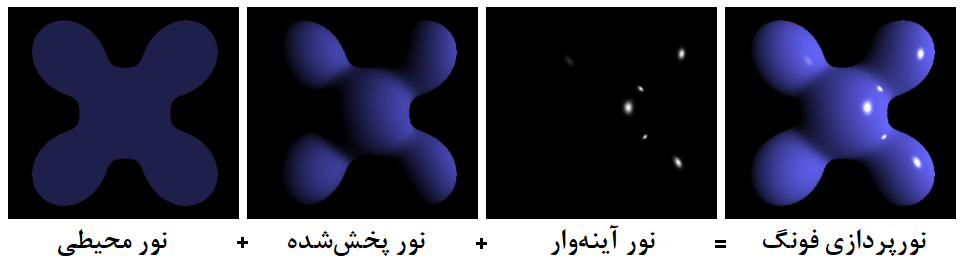
\includegraphics[width=\textwidth,height=\textheight,keepaspectratio]{Figures/Ch2/Phong_components.png}}

	\caption{مولفه‌های الگوریتم سایه‌زنی فانگ
    \cite{PhongShadingWikipedia}
    }
	\label{fig:PhongShadingWikipedia}
\end{figure}





\section{مدل اسکلتونی}

در انیمیشن‌های اسکلتونی از مدل‌های اسکلتونی استفاده می‌شود. هر مدل اسکلتونی از دو بخش مدل و اسکلت تشکیل‌شده‌است. 

\section{شبکه‌ی\protect\LTRfootnote{Mesh} چندضلعی}

در گرافیک کامپیوتری سه‌بعدی و مدل‌سازی جامد، شبکه چند‌ضلعی مجموعه‌ای از رئوس، لبه‌ها و وجوه است که شکل یک جسم چند‌وجهی را مشخص می‌کند.
وجوه معمولاً از مثلث‌ها (شبکه مثلثی)، چهار ضلعی‌ها (چهار گوشه)، یا دیگر چند ضلعی‌های محدب ساده
(
	\lr{n}
	ضلعی‌ها
)
تشکیل شده‌اند. دلیل استفاده از این نوع چند ضلعی‌ها آسان‌تر بودن به نمایش‌کشیدن آن‌ها در محیط سه‌بعدی است.
البته در حالت کلی اشیاء ممکن است از چندضلعی‌های مقعر و یا حتی چندضلعی‌های دارای سوراخ نیز تشکیل‌شده‌باشند.

اشیاء ایجادشده توسط مش‌های چند ضلعی باید انواع مختلفی از عناصر، از جمله رئوس، لبه‌ها، وجوه، چندضلعی‌ها و سطوح را در خود ذخیره کنند.
در بسیاری از نرم‌افزارهای سه‌بعدی، فقط رئوس، لبه‌ها و یکی از دو مورد وجوه یا چند‌ضلعی‌ها ذخیره می‌شوند.
در اکثر سیستم‌های رندر
\LTRfootnote{renderer}
فقط از وجوه سه‌ضلعی
(مثلث‌ها)
استفاده‌ می‌شود.
بنابراین در این حالت چند‌ضلعی‌های مدل، باید به شکل مثلث باشند. البته سیستم‌های رندر‌ ای وجود دارند که از چهارضلعی‌ها یا چندضلعی‌های با تعداد اضلاع بالاتر نیز پشتیبانی ‌می‌کنند و یا در لحظه این چندضلعی‌ها را به مجموعه‌ای از مثلث‌ها تبدیل می‌کنند که در این صورت باعث ‌می‌شود نیازی به ذخیره‌ی مش به شکل مثلثی نباشد.

بنابراین چهار قسمت اصلی یک مش چندضلعی، رئوس، لبه‌ها، وجوه و چندضلعی‌ها هستند. توضیح کوتاهی درباره‌ی هر کدام از این موارد را در زیر می‌توانیم مشاهده کنیم.

\subsection{راس}
راس‌ها معمولا یک موقعیت در فضای سه‌بعدی همراه با اطلاعات دیگر مانند رنگ، بردار نرمال و مختصات بافت را شامل می‌شوند. 
در راس‌های مربوط به مش‌های اسکلتونی اطلاعاتی مانند تعداد مفاصلی که بر روی این راس تاثیر می‌گذارند همراه با وزن تاثیرگذاری آن‌ها، می‌تواند اضافه شود.

\subsection{لبه}
ارتباط بین دو راس را لبه گویند.

\subsection{وجه}
مجموعه‌ای بسته از لبه‌ها را وجه گویند. وجه‌ها می‌توانند از سه لبه 
(وجه مثلثی)
یا از چهار لبه
(وجه چهارگوش)
تشکیل شده باشند.

\subsection{چندضلعی}
یک چندضلعی مجموعه‌ای همسطح از وجوه است.
در سیستم‌هایی که از وجه‌های چند ضلعی پشتیبانی می‌کنند، وجوه و چندضلعی‌ها یکسان هستند ولی در صورتی که سیستم مورد نظر تنها از سه یا چهار ضلعی‌ها پشتیبانی کند، در این صورت به چند ضلعی‌ها، مجموعه‌ای از وجوه گفته می‌شود.

\section{مدل}

مدل‌
\footnote{ گاهی به جای استفاده از واژه‌ی مدل، از واژه‌ی مش هم استفاده می‌شود.}
درواقع هر شئ‌ای است که در محیط سه‌بعدی قرار می‌گیرد و به تصویر کشیده ‌می‌شود. هر مدل می‌تواند از چند زیرمش تشکیل شود.
به عنوان مثال یک ماشین را درنظر بگیریم. موجودیت ماشین می‌تواند یک مدل باشد که در محیط سه‌بعدی قرار می‌گیرد. مدل ماشین می‌تواند از چند زیرمش مانند چرخ‌ها، لاستیک‌ها و بدنه‌ی ماشین تشکیل شود. دلیل وجود داشتن یک موجودیت کلی به اسم ماشین این است که یک ‌شخصی مانند طراح محیط و یا طراح مرحله ‌نمی‌خواهد هر بار که ماشینی را در محیط قرار دهد، تک تک زیرمش‌ها را به صورت دستی در صحنه وارد کند و در سر جای خودش قرار بدهد.


\section{زیرمش
\protect\LTRfootnote{Sub-Mesh}
}
چندضلعی‌های دارای یک نوع ماده
\LTRfootnote{Material}
را یک زیرمش گویند.
همانطور که اشاره شد، هر مدل از چند زیرمش تشکیل می‌شود. دلیل این تقسیم این است که در هر عملیات به تصویر کشیدن
\LTRfootnote{Render}
تنها یک ماده می‌تواند به تصویر کشیده شود. مثلا در مثال ماشین، قسمت‌های مختلف ماشین از ماده‌های مختلفی تشکیل می‌شود. به طور مثال چرخ ماشین می‌تواند از جنس آلومینیوم باشد، لاستیک چرخ از جنس پلاستیک باشد و یا حتی قسمت‌های داخلی ماشین مانند صندلی ماشین، از جنس چرم باشد.
بنابراین باید این قسمت‌ها به صورت جدا قرار گیرند تا بتوان هر قسمت را با توجه به ماده‌ی موردنظر آن به تصویر کشاند.

\section{ماده 
\protect\LTRfootnote{Material}
}
ماده‌ها شامل پارامتر‌های قابل تنظیمی هستند که با تنظیم آن‌ها، به گرافیک اعلام می‌شود که چگونه باید یک مثلث را به تصویر بکشد.
این پارامترها می‌توانند شامل موارد زیر باشند ولی محدود به آن نمی‌شوند

\begin{enumerate}
	\item میزان کدورت و شفافیت شئ
 	\item میزان براقی شئ
 	\item رنگ(بافت) شئ
 	\item سایه‌زنی پیکسلی یا راسی \protect\LTRfootnote{Vertex or Pixel shader}
\end{enumerate}


\section{بافت
\protect\LTRfootnote{Texture}
}
بافت یک تصویر دوبعدی و یا سه‌بعدی است که می‌تواند در ماده استفاده شود.
این تصاویر به عنوان ورودی در برنامه دریافت شده و پس از اینکه یک شناسه به آن ها تخصیص داده شد، در کارت گرافیک قرار می‌گیرند. ماده‌ها با استفاده از این شناسه می‌توانند در صورت لزوم به این بافت‌ها دستیابی پیدا کنند.


\section{اسکلت}

به مجمو‌عه ای از مفاصل که به صورت سلسله مراتبی به یکدیگر متصل می‌شوند، اسکلت گویند. پس از آنکه هنرمندان مدل شخصیت را طراحی می‌کنند در طی یک مرحله که به آن
\lr{Rigging}
گویند، ساختار سلسله مراتبی اسکلت را به وجود می‌آورند.
در انیمیشن‌ها درواقع این اسکلت‌ است که حرکت می‌کند و با حرکتش باعث حرکت مدل شخصیت می‌شود.


\section{
\lr{Skinning}
}

تا اینجا با دو مفهوم مدل و اسکلت آشنایی پیدا کردیم ولی نگفتیم که این دو چگونه به هم مرتبط می‌شوند.
به عملیاتی که طی آن مفاصل موجود در اسکلت به مدل متصل می‌شود 
\lr{skinning}
گویند.
طی این مرحله هر راس موجود در پوسته‌ی مش به یک یا چند مفصل متصل می‌شود.
برای اینکه چگونه رئوس مش، این مفاصل را دنبال کنند الگوریتم‌های مختلفی مطرح شده‌است که در فصل پیاده‌سازی به یکی آن‌ها اشاره ‌خواهد شد.


\section{ژست شخصیت}

ژست یک شخصیت نشان‌دهنده‌ی نحوه‌ی قرارگیری مفصل‌ها در اسکلت است. ژست‌های مختلف با دروان، حرکت یا تغییر اندازه‌ی مفاصل درون اسکلت به وجود می‌‌آیند.
همانگونه که اشاره شد، اسکلت یک مدل در مرحله‌ی 
\lr{Rigging}
به وجود می‌‌آید و در همین مرحله با استفاده از 
\lr{ Skinning}
 به مدل متصل می‌شود. زمانی که این عمل صورت می‌گیرد مدل در یک ژست به خصوص قرار دارد که به آن ژست حالت اتصال
\LTRfootnote{Bind Pose}
یا
ژست مرجع
\LTRfootnote{Reference Pose}
گویند.
به صورت کلی شخصیت در این حالت به صورتی ایستاده‌است که پاهایش کمی از هم باز است و 
بازو‌هایش به شکل حرف
\lr{T}
کشیده است. به همین جهت گاهی به ژست حالت اتصال،
ژست
\lr{T}
\LTRfootnote{T Pose}
هم گفته می‌شود.
این حالت خاص به این دلیل انتخاب می‌شود که اندام‌ها را از بدن دور نگه دارد و اینکار باعث می‌شود که 
فرایند اتصال رئوس به مفصل آسان‌تر شود.

همانگونه که اشاره‌‌شد مفاصل به صورت سلسله مراتبی به یکدیگر متصل هستند. یعنی نحوه‌ی 
قرارگیری آن‌ها متناسب با نحوه‌ی قرارگیری والدشان است.
این کار باعث می‌شود که مفاصل به صورت طبیعی حرکت کنند. یعنی در صورتی که والد حرکت کند، به واسطه‌ی 
آن فرزند نیز حرکت می‌کند.
زمانی که ژست شخصیت در این حالت والد، فرزندی قرار دارد به آن ژست محلی
\LTRfootnote{Local Pose}
گفته می‌شود. حالت دیگری نیز وجود دارد که موقعیت هر مفصل نسبت به فضای مختصاتی مدل 
درنظر گرفته می‌شود. به ژست شخصیت در این حالت ژست جهانی
\LTRfootnote{Global Pose}
گفته می‌شود.

\section{‌کلیپ‌های انیمیشنی}

در یک فیلم انیمیشنی، تمام بخش‌های یک صحنه قبل از ساخت هر انیمیشن به دقت برنامه‌ریزی می‌شود.
این شامل حرکات هر شخصیت، لوازم موجود در صحنه و حتی حرکات دوربین نیز می‌شود.
این بدان معنی است که کل صحنه را می‌توان به عنوان یک دنباله طولانی و پیوسته از فریم‌ها، متحرک ساخت.
در این حالت در صورتی که شخصیتی خارج از دوربین هستند لازم نیستند که متحرک شوند.

کلیپ‌های انیمیشنی متفاوت از این هستند. یک بازی، یک تجربه‌ی تعاملی است بنابراین نمی‌توان از قبل چگونه حرکت کردن شخصیت‌ها و رفتار آن‌ها را پیش‌بینی کرد.
حتی تصمیمات شخصیت‌های غیربازیکن کامپیوتری نیز می‌توانند تابعی از اقدامات غیر قابل پیش‌بینی بازیکن انسانی باشد.
به این ترتیب، کلیپ‌های انیمیشنی مربوط به بازی تقریبا هیچ‌گاه از مجموعه‌ای از فریم‌های طولانی و به هم پیوسته تشکیل نمی‌شوند.
درعوض، حرکت شخصیت بازی باید به تعداد زیادی حرکات ریز تقسیم شود. 
منظور از کلیپ‌های انیمیشنی این حرکات کوتاه و یکتا است.

بنابراین هر کلیپ به صورتی طراحی شده است که یک عمل کاملا مشخص را انجام دهد. برخی از این کلیپ‌ها به گونه‌ای طراحی شده اند که بتوان آن را به صورت حلقه شونده تکرار کرد.
به عنوان مثال چرخه‌ی راه‌رفتن یا دویدن می‌توانند از این نوع کلیپ‌ها باشند.
و حرکاتی مانند پریدن یا دست تکان دادن از نوعی هستند که تنها یک‌بار پخش می‌شوند.

بنابراین به طور کلی حرکات هر شخصیت بازی معمولا به هزاران کلیپ تقسیم می‌شود. \cite{GameEngineArchitecture}

\section{ترکیب انیمیشن}

اصطلاح ترکیب انیمیشن به هر تکنیکی اطلاق می‌شود که در آن بیش از یک کلیپ انیمیشن در ژست نهایی کاراکتر سهیم می‌شود.
به صورت دقیق تر در این عمل دو یا چند ژست برای ایجاد یک ژست خروجی برای اسکلت شخصیت، با یکدیگر ترکیب می‌شوند.
همانطور که در بخش قبل گفته شد، کلیپ‌های انیمیشنی، کلیپ‌های کوتاه و یکتایی هستند. با استفاده از روش ترکیب ‌می‌توان مجموعه‌ای از کلیپ‌های انیمیشنی را با یکدیگر ترکیب کرد تا مجموعه‌ی جدیدی از انیمیشن‌ها را بدون نیاز به ایجاد دستی و از پایه‌ی آن ها تولید کنیم.

به عنوان مثال، با ترکیب یک انیمیشن راه رفتن آسیب دیده با راه رفتن بدون آسیب دیدگی، می‌توانیم سطوح مختلفی از آسیب دیدگی در هنگام راه‌رفتن را به وجود آوریم.
از ترکیب می‌توان برای درون‌یابی بین حالات مختلف چهره، حالت‌های مختلف بدن و حالت‌های مختلف حرکتی استفاده کرد.
علاوه بر این می‌توان از آن برای یافتن یا حالت میانی بین دو حالت شناخته شده در زمان‌های مختلف نیز استفاده کرد. این‌کار زمانی استفاده می‌شود که بخواهیم ژست یک شخصیت را در نقطه‌ای از زمان پیدا کنیم که دقیقا با یکی از فریم‌های نمونه موجود در داده‌های انیمیشن مطابقت ندارد.
همچنین می‌توانیم از ترکیب موقتی انیمیشن برای انتقال هموار از یک انیمیشن به انیمیشن دیگر، با ترکیب تدریجی انیمیشن مبدا به مقصد در مدت زمان کوتاهی استفاده کنیم.